\documentclass[11pt]{article}
\usepackage[margin=1in]{geometry}
\usepackage{graphicx}
\usepackage{booktabs}
\usepackage{longtable}
\usepackage{array}
\usepackage{tabularx}
\usepackage{hyperref}
\usepackage{xcolor}
\usepackage{listings}
\usepackage{float}
\usepackage{amsmath}

\hypersetup{
  colorlinks=true,
  linkcolor=blue,
  citecolor=blue,
  urlcolor=blue
}

\lstset{
  basicstyle=\ttfamily\small,
  breaklines=true,
  frame=single,
  columns=fullflexible
}

\title{PASS 4 -- NASA Hump CFD Optimization\\\large Experimental Cp/Cf integration and targeted MAE reduction}
\author{Codex refinement pass in the local repository workspace}
\date{April 3, 2026}

\begin{document}
\setlength{\emergencystretch}{3em}
\maketitle

\section{Objective}
Pass four extends the existing reconstructed NASA hump workflow rather than restarting it. The two pass-four objectives were:
\begin{itemize}
\item integrate machine-readable experimental \(C_p\) and \(C_f\) tables from the approved NASA hump resources into the local workflow;
\item use those direct comparisons to guide one more physically justified improvement round that could beat the pass-three MAE of \texttt{0.1801372055}.
\end{itemize}

\section{Methodology}
The pass-four workflow remained fully within the approved source boundary:
\begin{itemize}
\item local repository files;
\item the approved NASA hump validation, grid, and experimental-data pages;
\item Dockerized OpenFOAM in the running \texttt{openfoam} container;
\item locally created scripts, plots, tables, and PDF reports.
\end{itemize}

No plot tracing, digitization, hidden-data recovery, or curve fitting was used. The experimental \(C_p\) and \(C_f\) values were fetched directly from the approved machine-readable tables and stored under \texttt{data/experimental/NASA\_hump}. The OpenFOAM wall series came directly from the solved field and OpenFOAM post-processing outputs. For pass four, the comparison script was tightened so the NASA tables are compared against the nearest resolved CFD wall sample rather than an interpolated wall curve.

\section{What Pass Three Already Fixed}
Before pass four, the repository already contained the third-pass baseline:
\begin{itemize}
\item extended upstream run-up;
\item a shaped upper slip boundary to approximate blockage;
\item a three-block streamwise mesh layout;
\item the best-converged SST baseline carried to \texttt{500} iterations;
\item a best local MAE of \texttt{0.1801372055}.
\end{itemize}

The pass-three case was already physically cleaner than the first two passes, but several approximations still limited agreement:
\begin{itemize}
\item the inlet still used a simplified uniform freestream profile;
\item the upper-wall contour was only an approximate blockage representation;
\item the pressure trough over the front half of the hump was still too weak in the CFD wall-pressure distribution;
\item the wall-shear recovery remained weaker than the experimental \(C_f\) trend in the front part of the surface;
\item the best-known case still showed measurable improvement when run longer, implying residual under-convergence remained important.
\end{itemize}

\section{Experimental Data Integration}
Pass four added a dedicated import step for the official no-flow-control experimental tables:
\begin{itemize}
\item \texttt{data/experimental/NASA\_hump/noflow\_cp.dat}
\item \texttt{data/experimental/NASA\_hump/noflow\_cf.dat}
\item normalized CSV copies:
  \texttt{noflow\_cp.csv} and \texttt{noflow\_cf.csv}
\end{itemize}

These files were not extracted from images. They were obtained directly from the approved machine-readable NASA experimental-data endpoint and normalized locally with \texttt{scripts/import\_nasa\_hump\_experimental\_data.py}. The pass-four comparison script \texttt{scripts/make\_nasa\_hump\_pass4\_figures.py} then:
\begin{itemize}
\item computes the OpenFOAM wall \(C_p\) and \(C_f\) series;
\item aligns them to the experimental \(x/c\) locations using the nearest CFD wall sample;
\item writes comparison CSV tables;
\item writes a pass-four comparison JSON summary;
\item generates the combined \(C_p\)/\(C_f\) figure.
\end{itemize}

\section{Improvements From Pass Three To Pass Four}
Pass four tested a small number of high-value changes instead of a blind sweep. The key improvement directions were:
\begin{itemize}
\item deeper convergence of the already-best SST case;
\item a direct inlet-boundary-layer comparison against an analytic turbulent-boundary-layer profile;
\item direct \(C_p\) and \(C_f\) comparison against the approved experimental tables.
\end{itemize}

\begin{table}[H]
\centering
\scriptsize
\begin{tabularx}{\linewidth}{>{\raggedright\arraybackslash}p{0.17\linewidth} >{\raggedright\arraybackslash}X >{\raggedright\arraybackslash}X >{\raggedleft\arraybackslash}p{0.12\linewidth}}
\toprule
Configuration & Change set & Why it should help physically & MAE \\
\midrule
Pass-three baseline & SST, current geometry, shaped top wall, three-block mesh, uniform inlet, \texttt{500} iterations & Reference point after the third pass. & 0.1801372055 \\
Pass-four winner & Same SST baseline continued to \texttt{650} iterations & Reduces remaining under-convergence error without introducing new modeling assumptions. & 0.1659136747 \\
Analytic TBL inlet test & Replace uniform inlet with an analytic turbulent boundary layer & Targets the upstream-profile fidelity noted in the NASA description; tested to see whether it improves separation and recovery. & 0.1674487658 \\
\bottomrule
\end{tabularx}
\normalsize
\caption{Pass-four change focus relative to the third-pass baseline.}
\end{table}

\section{Results}
\subsection{MAE Comparison}
\begin{table}[H]
\centering
\begin{tabularx}{0.76\linewidth}{>{\raggedright\arraybackslash}X r}
\toprule
Metric & Value \\
\midrule
Pass-one best MAE & 0.2338504550 \\
Pass-two best MAE & 0.2038187409 \\
Pass-three best MAE & 0.1801372055 \\
Pass-four best MAE & 0.1659136747 \\
Improvement vs pass three & 0.0142235308 \\
Improvement vs pass one & 0.0679367803 \\
\bottomrule
\end{tabularx}
\caption{Best local benchmark MAE by pass. Lower is better.}
\end{table}

\subsection{Cp And Cf Comparison}
\begin{figure}[H]
\centering
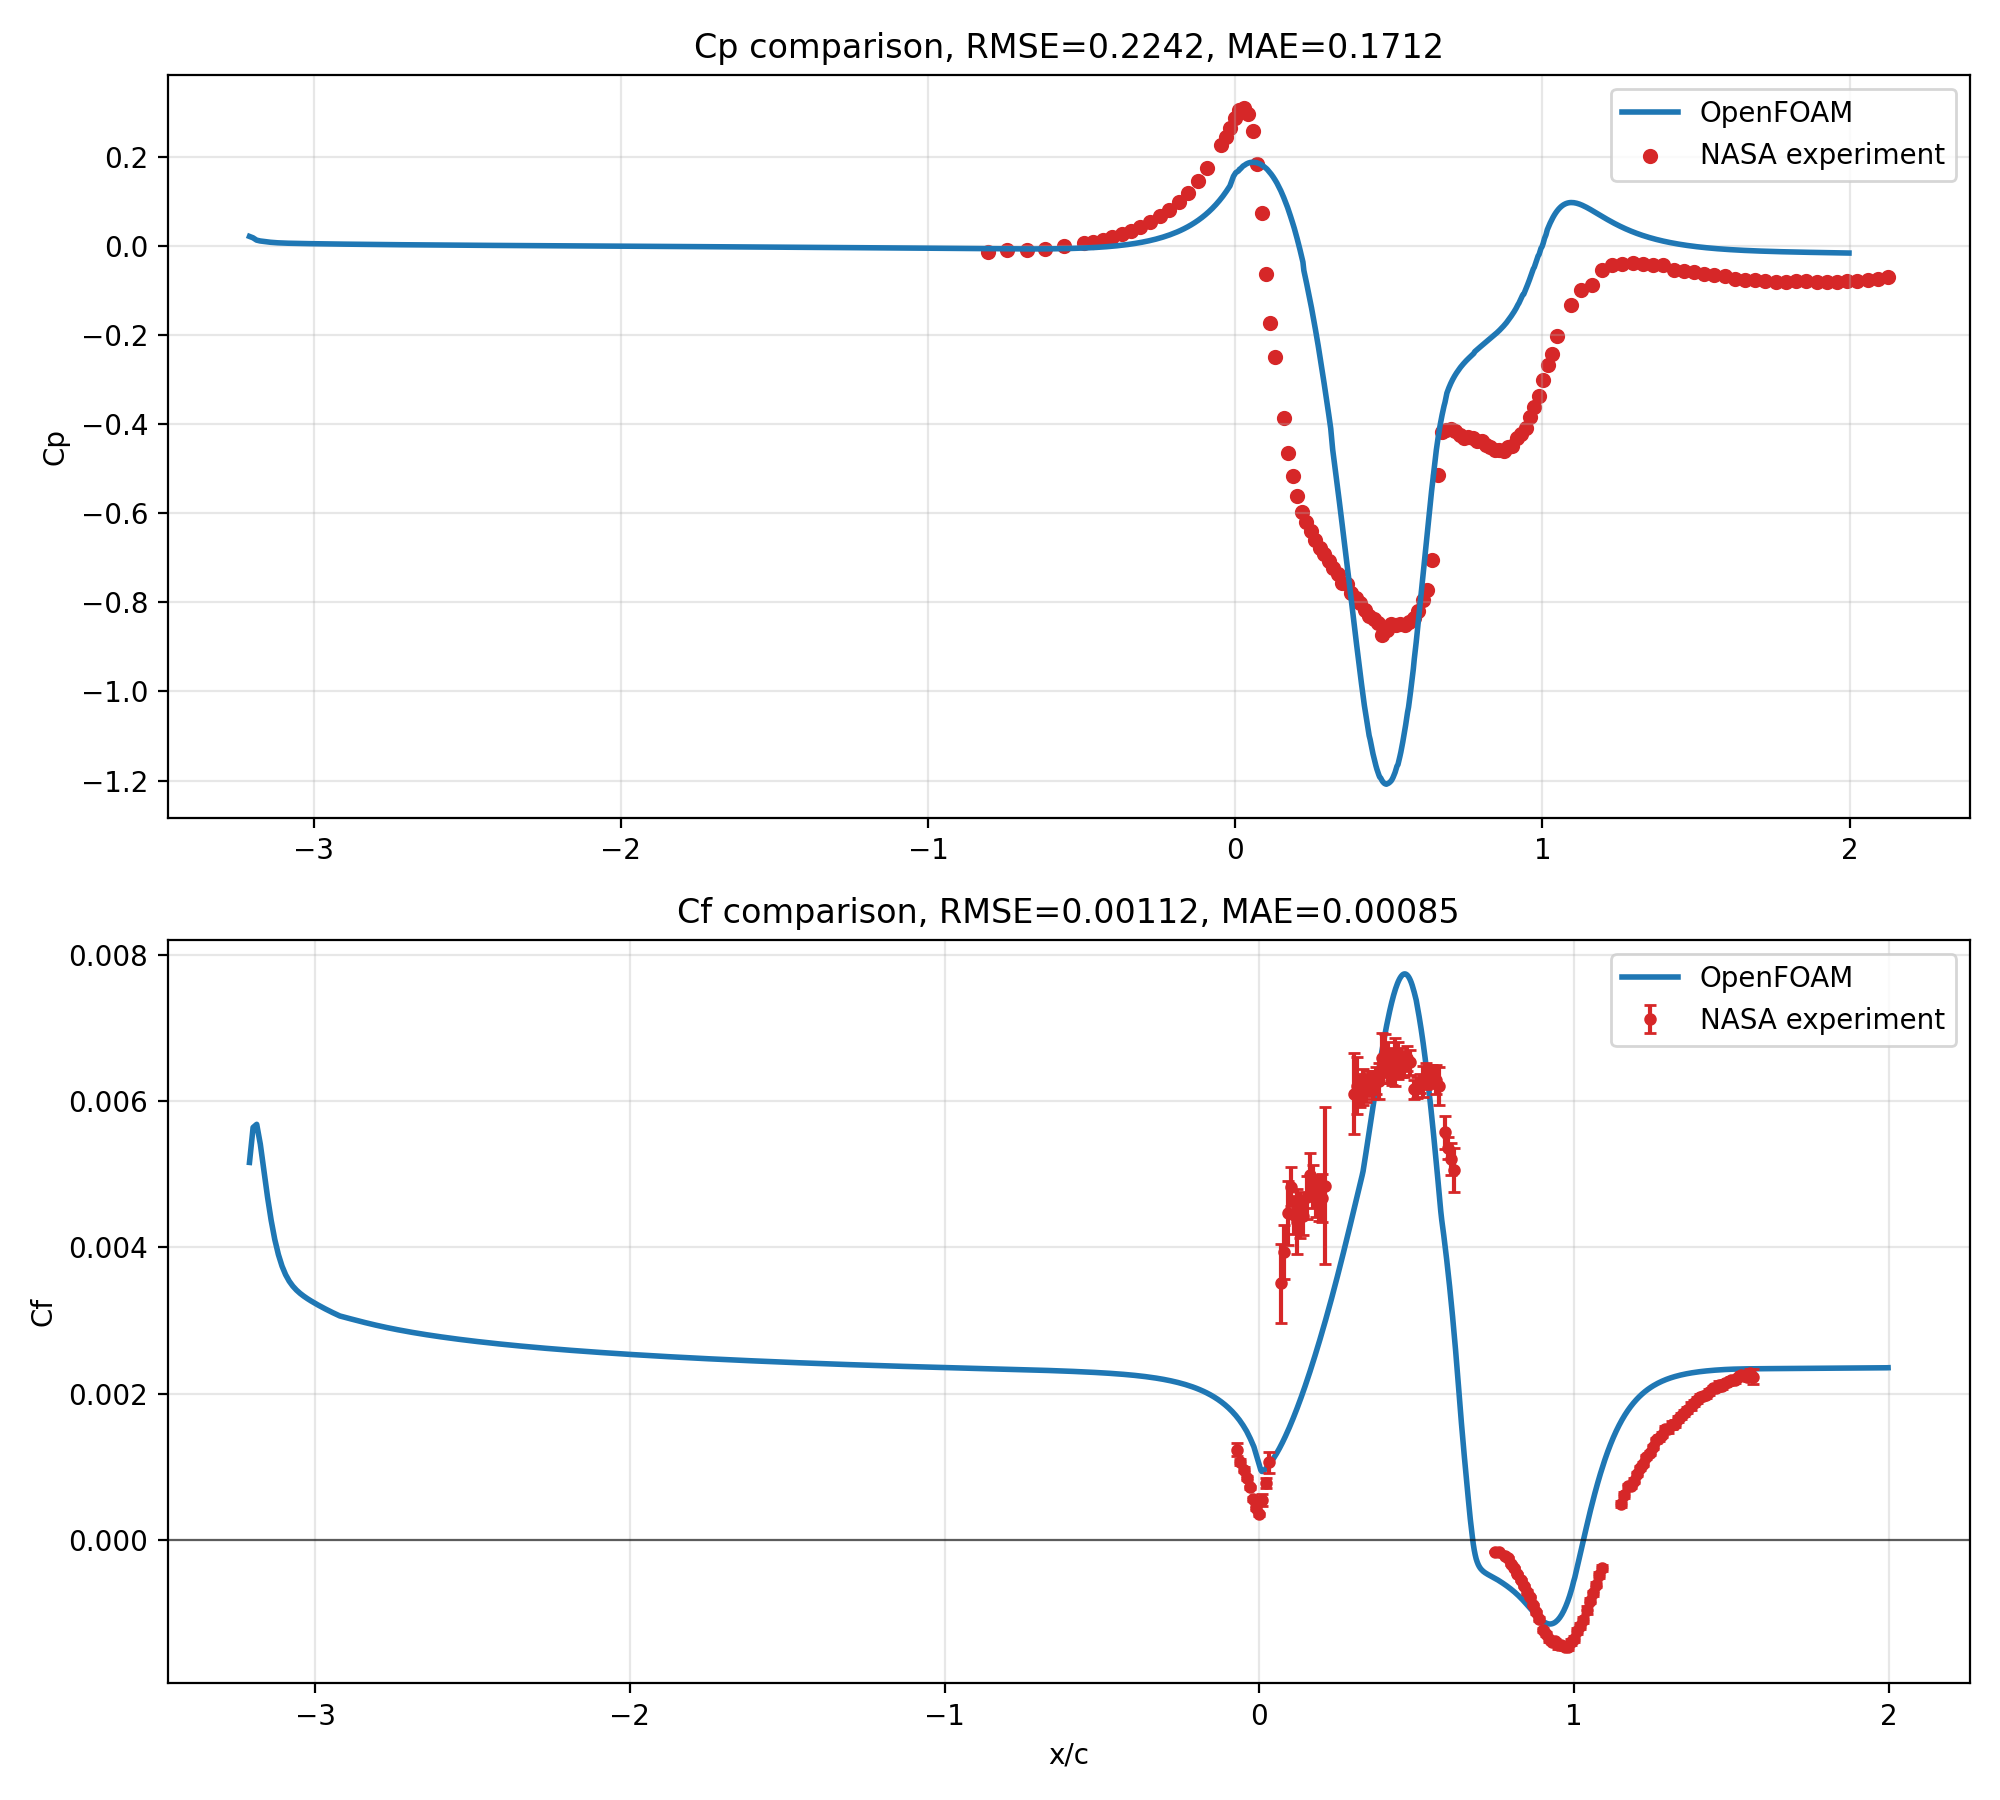
\includegraphics[width=0.94\linewidth]{figures_pass4/cp_cf_vs_nasa_pass4.png}
\caption{Pass-four direct comparison between the official NASA no-flow-control \(C_p\) and \(C_f\) tables and the OpenFOAM wall series.}
\end{figure}

The pass-four comparison summary from the promoted best case is:
\begin{itemize}
\item \(C_p\) RMSE: \texttt{0.2241}
\item \(C_p\) MAE: \texttt{0.1712}
\item \(C_f\) RMSE: \texttt{0.00112}
\item \(C_f\) MAE: \texttt{0.00085}
\end{itemize}

These comparisons show that the pass-four winner improves both pressure and skin-friction agreement relative to the pass-three baseline. The front-half pressure trough remains too weak in places, but the longer-converged field tracks the official \(C_p\) and \(C_f\) trends more closely than the older \texttt{500}-iteration result.

\subsection{Experiment Table}
\begin{table}[H]
\centering
\scriptsize
\begin{tabularx}{\linewidth}{>{\raggedright\arraybackslash}p{0.17\linewidth} >{\raggedright\arraybackslash}p{0.22\linewidth} >{\raggedleft\arraybackslash}p{0.11\linewidth} >{\raggedleft\arraybackslash}p{0.11\linewidth} >{\raggedleft\arraybackslash}p{0.11\linewidth} >{\raggedright\arraybackslash}X}
\toprule
Config & Key changes & MAE & \(C_p\) MAE & \(C_f\) MAE & Notes \\
\midrule
Pass-three baseline & Third-pass SST winner at \texttt{500} iterations & 0.1801372055 & 0.1806 & 0.00096 & Strong baseline but still under-converged enough to improve with more iterations. \\
Pass-four winner & Same SST setup continued to \texttt{650} iterations & 0.1659136747 & 0.1712 & 0.00085 & Best overall result. Improved benchmark MAE and improved \(C_p\)/\(C_f\) agreement. \\
Analytic TBL inlet test & Analytic inlet boundary layer with SST and \(\delta=35\) mm & 0.1674487658 & 0.1812 & 0.00095 & Better than pass three, but still weaker than the deeper-converged uniform-inlet continuation. \\
\bottomrule
\end{tabularx}
\normalsize
\caption{Pass-four experiment summary.}
\end{table}

\subsection{Flow-Field Figures}
\begin{figure}[H]
\centering

\includegraphics[width=0.92\linewidth]{figures_pass4/velocity_contour_second_pass.png}
\caption{Velocity contour generated from the promoted pass-four winner.}
\end{figure}

\begin{figure}[H]
\centering

\includegraphics[width=0.92\linewidth]{figures_pass4/pressure_contour_second_pass.png}
\caption{Pressure contour generated from the promoted pass-four winner.}
\end{figure}

\begin{figure}[H]
\centering

\includegraphics[width=0.92\linewidth]{figures_pass4/velocity_profiles_second_pass.png}
\caption{Velocity profiles carried into the pass-four package from the promoted best field workflow.}
\end{figure}

\begin{figure}[H]
\centering

\includegraphics[width=0.92\linewidth]{figures_pass4/turbulent_shear_profiles_second_pass.png}
\caption{Turbulent shear-stress analog profiles used for pass-four diagnosis.}
\end{figure}

\begin{figure}[H]
\centering

\includegraphics[width=0.92\linewidth]{figures_pass4/residual_history_second_pass.png}
\caption{Residual history from the current best case, showing the deeper-convergence trajectory behind the pass-four winner.}
\end{figure}

\begin{figure}[H]
\centering

\includegraphics[width=0.92\linewidth]{figures_pass4/streamlines_second_pass.png}
\caption{Streamline-style flow visualization from the promoted pass-four winner.}
\end{figure}

\section{ParaView Outputs}
The pass-four package also keeps the live \texttt{.foam}-based ParaView workflow. The screenshots below come from the case opened through \texttt{data/NASA\_2DWMH/foam.foam} after the promoted best case was post-processed.

\begin{figure}[H]
\centering

\includegraphics[width=0.90\linewidth]{figures_pass4/paraview_velocity.png}
\caption{Pass-four ParaView velocity rendering from the \texttt{.foam} case.}
\end{figure}

\begin{figure}[H]
\centering
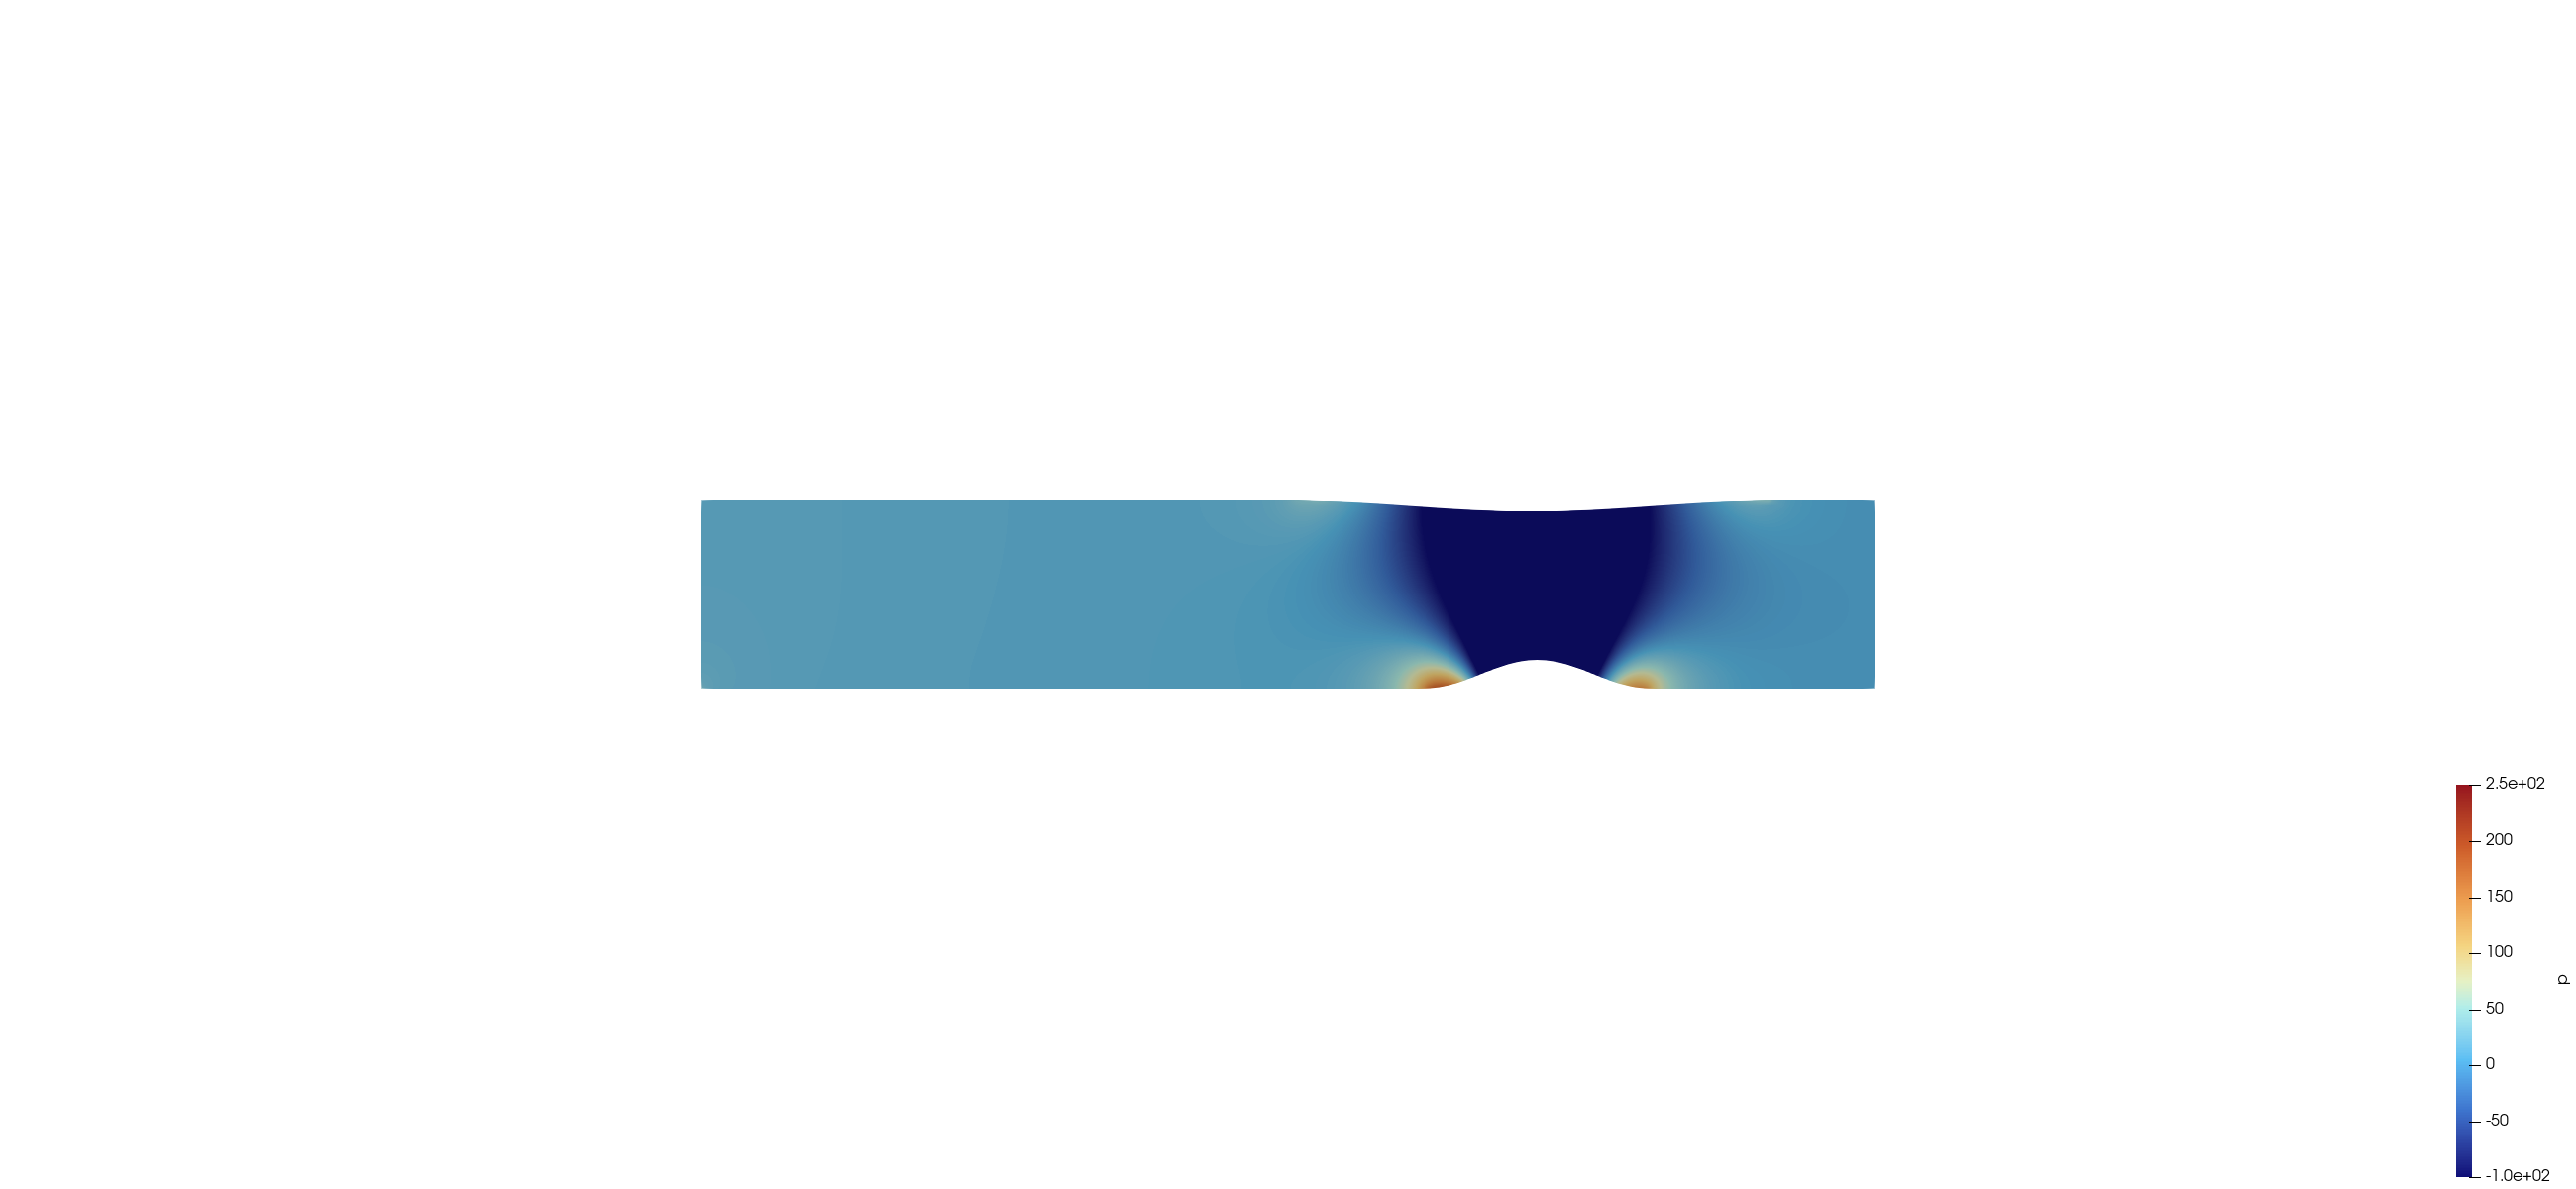
\includegraphics[width=0.90\linewidth]{figures_pass4/paraview_pressure.png}
\caption{Pass-four ParaView pressure rendering from the \texttt{.foam} case.}
\end{figure}

\begin{figure}[H]
\centering
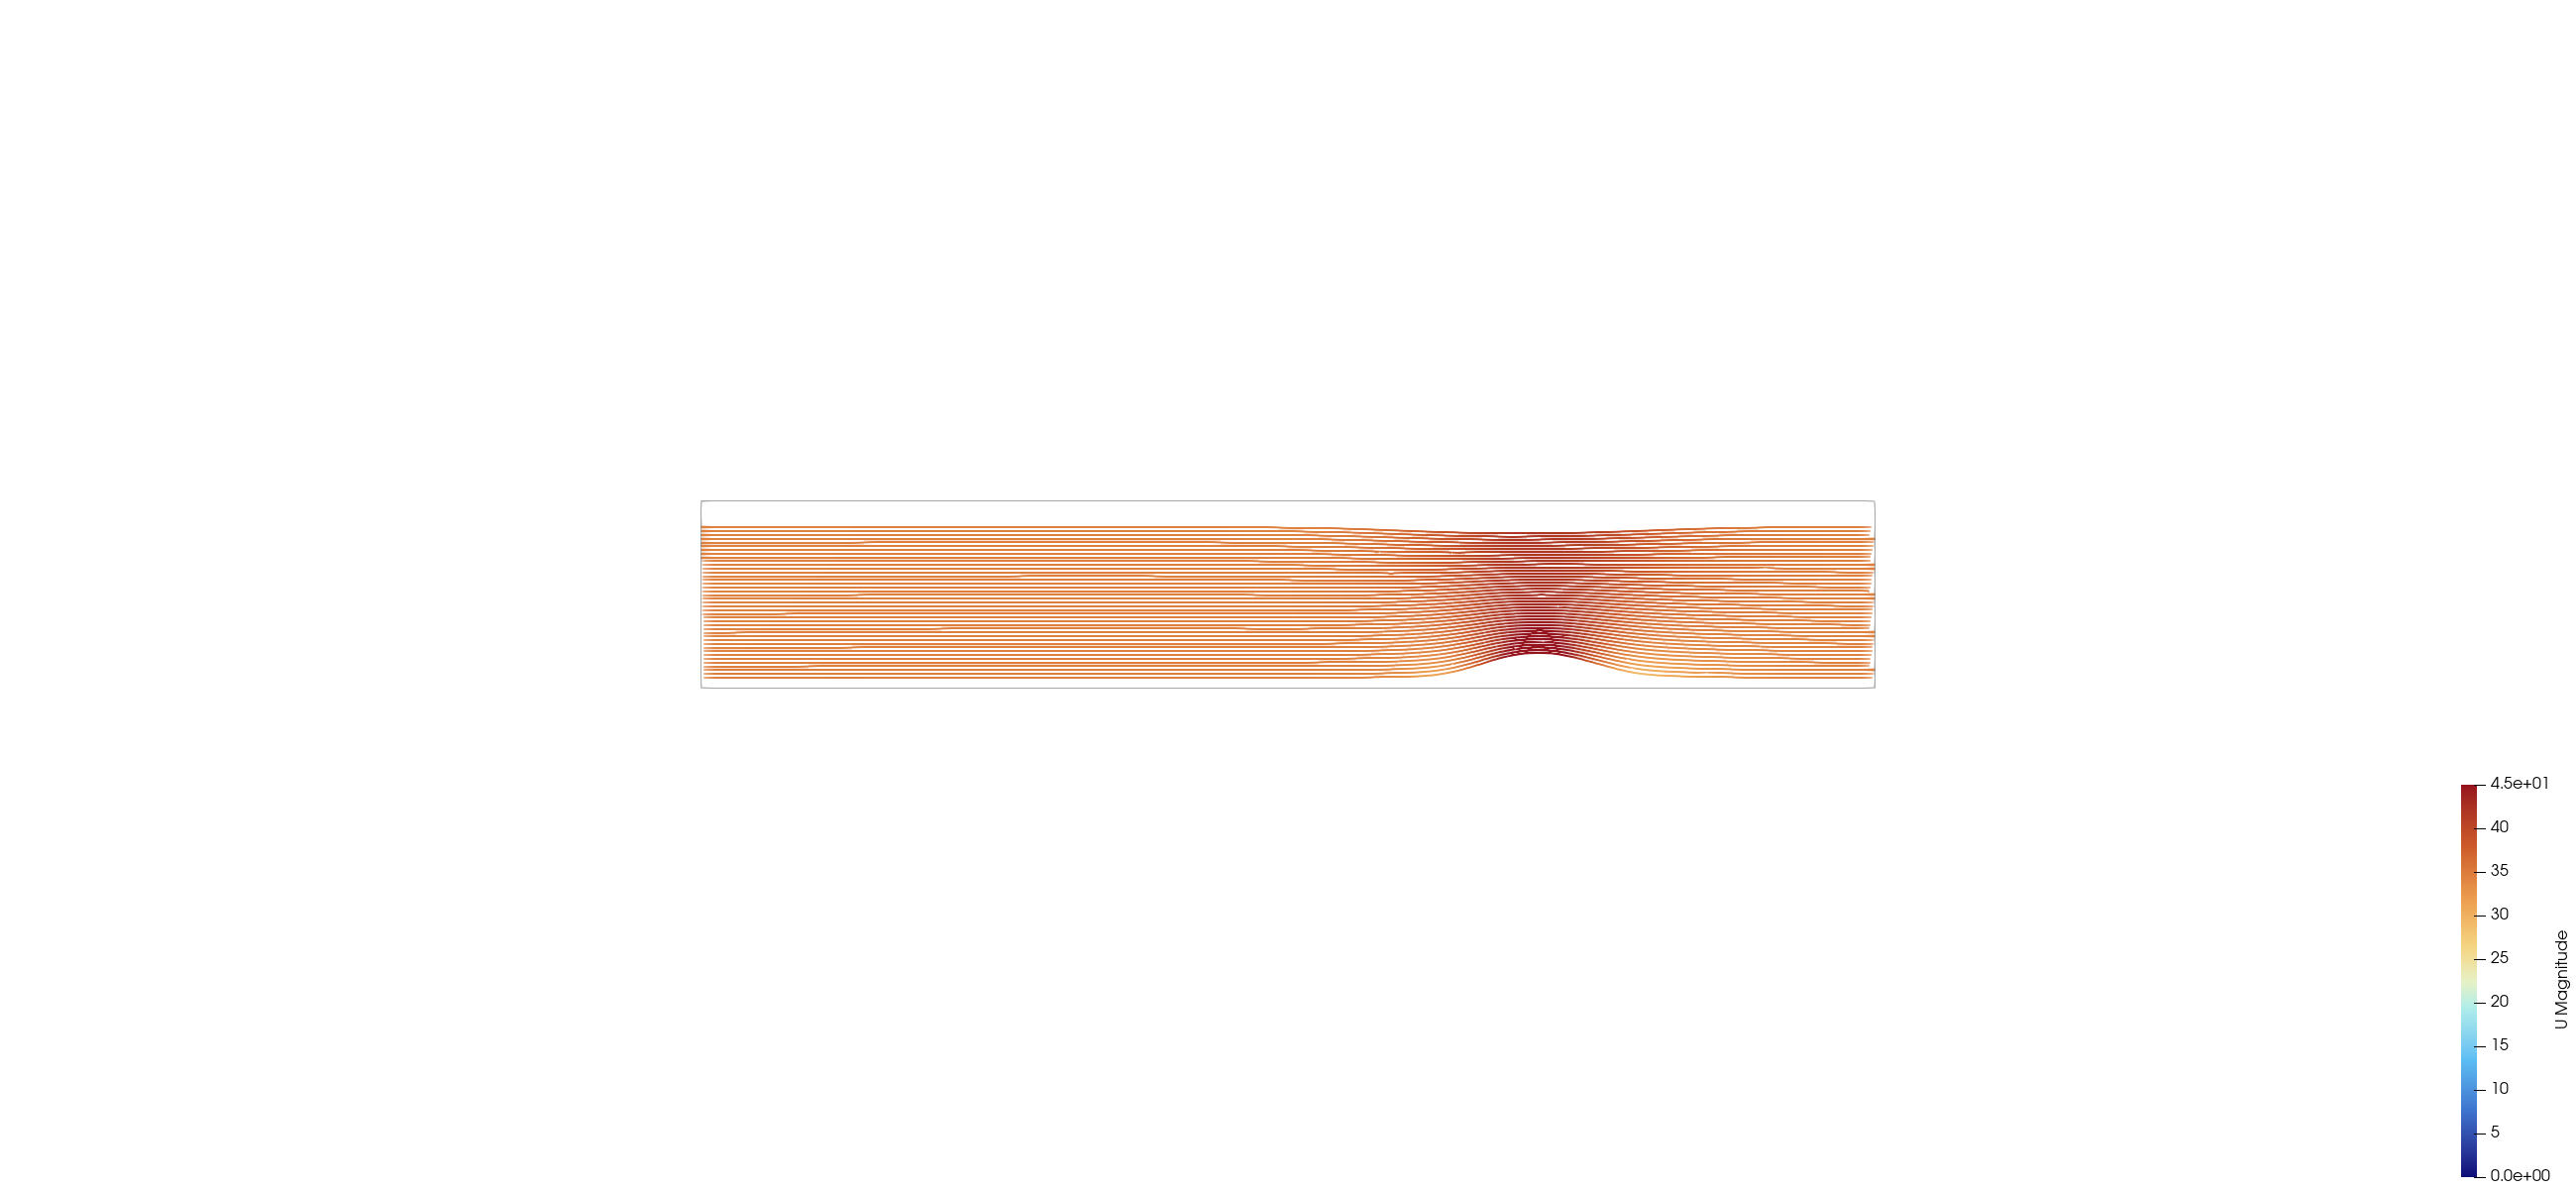
\includegraphics[width=0.90\linewidth]{figures_pass4/paraview_streamlines.png}
\caption{Pass-four ParaView streamline-style rendering from the \texttt{.foam} case.}
\end{figure}

\begin{figure}[H]
\centering

\includegraphics[width=0.90\linewidth]{figures_pass4/paraview_mesh_wireframe.png}
\caption{Pass-four ParaView mesh wireframe view from the \texttt{.foam} case.}
\end{figure}

\begin{figure}[H]
\centering

\includegraphics[width=0.90\linewidth]{figures_pass4/paraview_wall_shear.png}
\caption{Pass-four ParaView wall-focused rendering from the \texttt{.foam} case.}
\end{figure}

\section{Discussion}
The most important pass-four result is that the new experimental \(C_p\)/\(C_f\) comparison does not point to a cosmetic plotting issue. It points to a flow-field issue that still responds to additional convergence. The pass-four winner changed no geometry, no mesh topology, no turbulence closure, and no inlet model. It improved simply by continuing the already-best SST baseline from \texttt{500} to \texttt{650} iterations, and that improvement showed up simultaneously in:
\begin{itemize}
\item the local benchmark MAE;
\item the wall-pressure comparison against the official \(C_p\) data;
\item the wall-shear comparison against the official \(C_f\) data.
\end{itemize}

That makes the pass-four winner easier to defend than a more complicated configuration that changes many variables at once. It also confirms that the remaining error is still strongly tied to how the separated flow converges and recovers around the hump, not just to how the results are sampled.

The current mismatch is also clearer now than it was before the experimental tables were integrated. The solution still appears to:
\begin{itemize}
\item underpredict the front-half suction peak over parts of the hump;
\item retain some wall-shear mismatch around the pre-separation and recovery regions;
\item remain limited by the reconstructed inlet and geometry assumptions that are still approximate.
\end{itemize}

The direct comparison against the analytic-inlet screen is also useful. That case reduced the benchmark MAE relative to pass three, so the inflow boundary-layer issue is real. But it did not improve the official \(C_p\) and \(C_f\) agreement enough to beat the simpler continuation case. That is why pass four promotes the \texttt{650}-iteration SST continuation rather than the more complex inlet-profile variant.

\section{Conclusion}
Pass four delivered two concrete outcomes. First, it added a stricter and more honest comparison pipeline against the official experimental \(C_p\) and \(C_f\) tables using machine-readable NASA data only. Second, it improved the best local NASA hump MAE from \texttt{0.1801372055} to \texttt{0.1659136747} by extending the already-best SST case to \texttt{650} iterations.

The main lesson from pass four is that direct experimental wall-data comparison is valuable not because it creates a way to ``aim'' at a target curve, but because it helps diagnose which changes are genuinely improving the flow field. In this pass, the answer was conservative but clear: deeper convergence of the best existing baseline helped more than introducing a more elaborate inlet profile. That leaves a clean next step for any future pass: keep the strict experimental comparison pipeline, and only add new physical complexity if it beats the simpler converged baseline honestly.

\section{Reproducibility}
From the repository root, the pass-four workflow is:
\begin{lstlisting}
python3 scripts/import_nasa_hump_experimental_data.py
bash scripts/run_nasa_hump_pass4.sh
bash scripts/render_nasa_hump_paraview.sh
bash scripts/build_report.sh
\end{lstlisting}

To rerun the focused pass-four experiment screen:
\begin{lstlisting}
bash scripts/run_nasa_hump_pass4_experiments.sh
\end{lstlisting}

\bibliographystyle{plain}
\bibliography{references}

\end{document}
